%
%    F U K U D A
%


\documentclass[10pt,b5paper,papersize,dvipdfmx]{jsbook}
% 会誌は B5 サイズです

\usepackage{vuccaken}
\usepackage{vuccaken2019}
\usepackage{cases}    %後でvuccaken2019.styに追加!

% スタイルファイルの読み込みや自作マクロは、
% 最終的には vuccaken2019.sty の中に書いてください。
% とりあえずはここに書いてもらって構いません。


\begin{document} % 以下本文

% - - - - - - - - - - - - - - - - - - - - - - - - %
\kaishititle%
  {理工学部物理科学科}% 所属
  {福田大和}% name
% - - - - - - - - - - - - - - - - - - - - - - - - %

% \setcounter{tocdepth}{2} % 目次にどこまで表示するか
% \tableofcontents % 目次出力
% \clearpage % 改ページ

\section{はじめに}
前半で電磁気学の概要をかなーーーーーーーーーーーり駆け足で説明し、後半では私個人の考えを展開していきます。あらかじめ注意して頂きたいのですが、この説明は私の説明しやすい順番で、私の理解が及ぶ範囲で説明しています。具体的には、多くの電磁気学の教科書はクーロンの法則などの、あまり電磁気学に触れたことのない方にも直感的に分かりやすい関係式から初めて、マクスウェル方程式を導き、云々、という展開が一般的かと思います。しかし、今回は初めに電磁気学全てを支配するマクスウェル方程式を提示し、種々の関係式を導くという順序です。この順序にした理由は二つあり、一つは私が前述したような一般的な説明に馴染めないということ。ありていに言うと、うまく説明できる自信がない為です。もう一つは、ここでの主題である磁気単極子についての議論をするときに、この順序で説明した方がすんなり受け入れていただけるのではと考えたからです。あらかじめ断っておきますが、間違っている可能性も十二分にあり得ますのでそのことに留意してお読みいただければ幸いです。

\section{電磁気学}
\subsection{マクスウェル方程式}
早速始めていきます。兎にも角にも、まずはマクスウェル方程式を見て頂きましょう。
\subsubsection{積分形}

以上の四つがマクスウェル方程式と呼ばれる、電磁気学全てを支配する方程式達です。

\subsubsection{微分形}

\subsection{静電場}
\subsection{静磁場}
\subsection{時間変化}
\subsection{}

\section{オリジナル理論展開したい(願望)}
\subsection{なるようになーれー}

\section{参考文献}
\renewcommand{\labelenumi}{[\arabic{enumi}]} % [1],[2],...
\begin{enumerate}
\item 小宮山 進・竹川 敦,『マクスウェル方程式から始める電磁気学』,裳華房,2016/9/15 第二版
\item (複数ある場合は追加)
\item @vuccaken, 物科研HP, \url{rp2017xy.starfree.jp}, 2019.
\end{enumerate}
\renewcommand{\labelenumi}{\arabic{enumi}.} % default

\end{document}


%\subsubsection{テイラー展開}
%三角関数および指数関数のテーラー展開は次の通りである:
%\begin{align}
%    \cos x &= \sum_{n=0}^\infty \frac{(-1)^n}{(2n)!} x^{2n}, \label{eq:cos}\\
%    \sin x &= \sum_{n=0}^\infty \frac{(-1)^n}{(2n+1)!} x^{2n+1}, \label{eq:sin}\\
%    e^x &= \sum_{n=0}^\infty \frac{1}{n!} x^n. \label{eq:exp}
%\end{align}
%
%
%\subsubsection{オイラーの公式}
%(\ref{eq:cos}),(\ref{eq:sin}),(\ref{eq:exp})式より
%\begin{align*}
%    e^{ix} = \sum_{n=0}^\infty \frac{1}{n!} (ix)^n
%    &= \sum_{n=0}^\infty \frac{(-1)^n}{(2n)!} x^{2n} + i\sum_{n=0}^\infty \frac{(-1)^n}{(2n+1)!} x^{2n+1} \\
%    &= \cos x + i\sin x
%\end{align*}
%よってオイラーの公式 $ e^{ix} = \cos x + i\sin x $ が示された。
%
%
%\subsubsection{ギリシャ文字、数学記号}
%ギリシャ文字とか記号は$\Gamma^\alpha_{\ \beta\gamma}, \Psi(x), \cos\theta, \sin^2\phi$や$\infty, \equiv, \approx, \to, \iff, \times, %\cdots, \le$のように書きます。
%変換でα, β, ∞, ×みたいにしないこと!
%
%
%\subsection{グラフや画像の挿入}
%\TeX はこれがめんどい。figure環境ごとコピペして使おう。
%
%\begin{figure}[htbp]
%  \centering
%  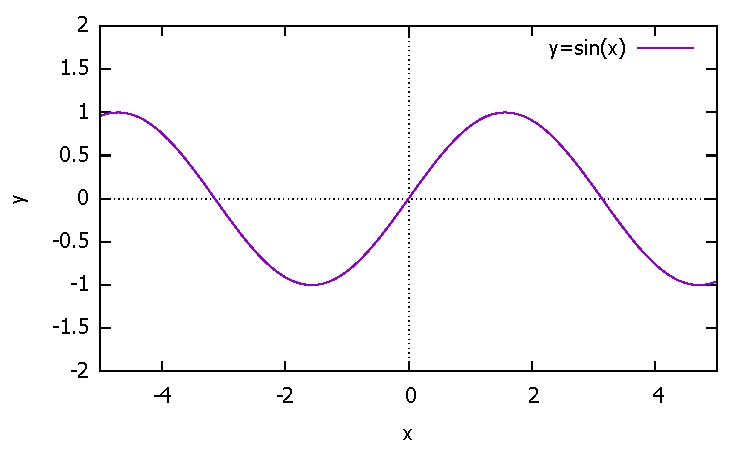
\includegraphics[width=10cm]{img/fig-sin.pdf}
%  \caption{$y=\sin x$のグラフ。gnuplotで作成した。}
%  \label{fig:sin}
%\end{figure}
%
%図\ref{fig:sin}より、sinが{\bfseries うねうね}であることがわかる。

%
%\subsection{ascmacパッケージ}
%枠で囲める。
%\begin{itembox}[l]{定義(ゼータ関数)}
%  $\Re(s) > 1$である任意の複素数$s$について、リーマンのゼータ関数$\zeta (s)$を以下のように定義する:
%  \begin{align*}
%    \zeta (s) := \sum_{n=1}^\infty \frac{1}{n^s}
%    \equiv \frac{1}{1^s} + \frac{1}{2^s} + \frac{1}{3^s} + \frac{1}{4^s} + \cdots
%  \end{align*}
%\end{itembox}

%
%\subsection{作図}
%\LaTeX と連携できるものとしては、picture環境やTi{\itshape k}ZやgnuplotやInkscapeなど色々な方法がありますが、ここではキーワードを挙げるに留めておきます。
%手描きを写真で撮ったり\footnote{明るさとコントラストをあげればそこそこキレイになる。}、パワポとかで作っても良いと思います\footnote{jpegは圧縮されて汚いので、pngか、ベクター形式のsvgとかpdfで作ると良い。}。

%
%\subsection{ソースコード}
%プログラムなどのソースコードを表示するにはlisting.styを使えばキレイに出力できますが、日本語に厳しい。そこで誰かが作ったplistings.styを代わりに使ってください。使い方はlisting.styと同じなので、そちらをキーワードにしてググってくだ
